Pierwsz� propozycj� by�o najbardziej kompleksowe rowi�zanie, czyli "Ground station". Jednym z proponowanych modeli by�: DJI iPad Ground Station w/Bluetooth Module. Cechami wyr�niaj�cymi go by�y:

\begin{itemize}
\item nadajnik i odbiornik 2.4 Ghz,
\item modu� Bluetooth i oprogramowanie PC Ground Station umo�liwiaj�ce nawigacje,
\item dane typu stan baterii, wysoko�� itp.,
\item zasieg BT w pomieszczeniach do 350m,
\item moc 125mW,
\item cena 199 USD.
\end{itemize}

\begin{figure}[H]
\centering
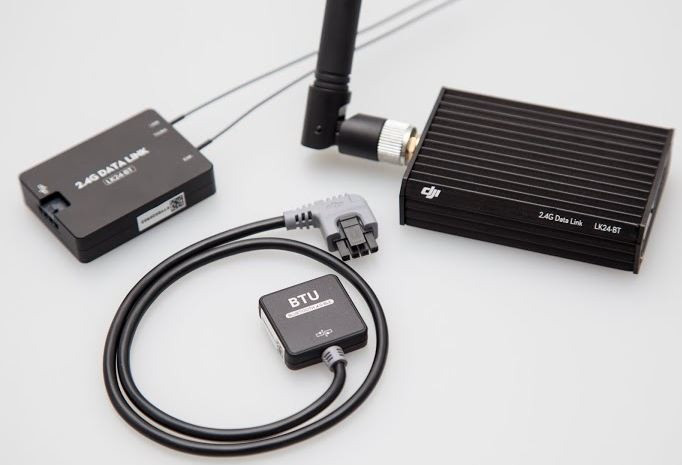
\includegraphics[width=0.7\textwidth]{./grafika/ground1.png}
\caption[DJI Ground Station]{}
\end{figure}

Kolejnym zaproponowanym rozwi�zaniem by�: Quanum FPV Ground Station with 8? Monitor and Voltage Display, kt�ry cechowa� si� nastepuj�cymi elementami:

\begin{itemize}
\item rozwi�zanie FPV - monitor LCD,
\item gotowe wyprowadzenia (kable, z�acza) do pod�aczenia anteny, sygna�u video, modu�u radiowego itp.,
\item nie zawiera �adnych odbiornik�w,
\item cena ok. 130 EUR,
\end{itemize}

\begin{figure}[H]
\centering
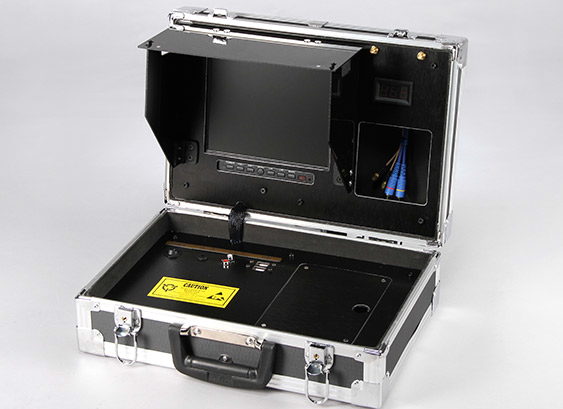
\includegraphics[width=0.7\textwidth]{./grafika/ground2.png}
\caption[Quanum FPV Ground Station]{}
\end{figure}

Ostatni� alternatyw� jest QGroundControl. Prezentowane rozwi�zanie nie tyle jest samodzielnym produktem co niezale�nym oprogramowaniem dedykowanym dla stacji PIXHAWK. Pakiet zawiera nast�puj�ce elementy:

\begin{itemize}
\item Open Source - protok� MAVLink,
\item Linux Support,
\item mapy 2D/3D,
\item �atwe ustawianie punkt�w przelotu i manipulacja w locie,
\item przedstawianie danych telemetrycznych w czasie rzeczywistym,
\item wsparcie dla UDP i komunikacji radiowej,
\item wsparcie dla autopilota, m.in. pxIMU,
\item wsparcie dla transmisji video,
\item obs�uga wielu pojazd�w jednoczesnie.
\end{itemize}

\begin{figure}[H]
\centering
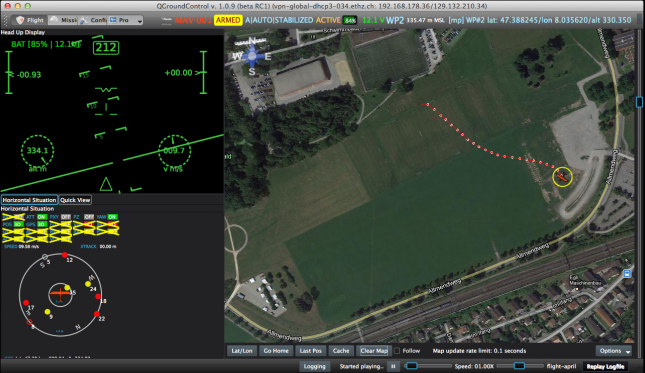
\includegraphics[width=0.7\textwidth]{./grafika/ground3.png}
\caption[QGroundControl]{}
\end{figure}
